\documentclass{article}
    \usepackage{url}
    \usepackage{cite}
    \usepackage{float}   
    \usepackage{xcolor}
    \usepackage{lscape}
    \usepackage{amssymb}
    \usepackage{titling}
    \usepackage{pdfpages}
    \usepackage{enumitem}
    \usepackage{graphicx}
    \usepackage{hyperref}
    \usepackage{fancybox}
    \usepackage{fancyvrb}
    \usepackage{enumerate}
    \usepackage{pdflscape}
    \usepackage{afterpage}
    \usepackage{listings,lstautogobble}    
    \usepackage[margin=0.8in]{geometry}
    \usepackage[nottoc,notlot,notlof]{tocbibind}
    \renewcommand\maketitlehookd{\vfill\null}
    \renewcommand\maketitlehooka{\null\mbox{}\vfill}

    \newcommand\backgroundimage{
        \put(-5,0){
        \parbox[b][\paperheight]{\paperwidth}{
        \vfill
        \centering
        %
\includegraphics[height=\paperheight]{Images/background.jpg}
        \vfill
    }}}

    % Stole code from: https://tex.stackexchange.com/questions/83882/how-to-highlight-python-syntax-in-latex-listings-lstinputlistings-command

    % Default fixed font does not support bold face
    \DeclareFixedFont{\ttb}{T1}{txtt}{bx}{n}{12} % for bold
    \DeclareFixedFont{\ttm}{T1}{txtt}{m}{n}{12}  % for normal

    \definecolor{deepblue}{rgb}{0,0,0.5}
    \definecolor{deepred}{rgb}{0.6,0,0}
    \definecolor{deepgreen}{rgb}{0,0.5,0}

    % SQL style for highlighting
    \lstset{
        language=SQL,
        basicstyle=\small,
        commentstyle=\color{gray},
        otherkeywords={self},
        keywordstyle=\ttb\color{deepblue},
        stringstyle=\color{deepgreen},
        numbers=left,
        numberstyle=\small,
        breaklines=true,
        frame=tb,
        showstringspaces=false,
        autogobble=true
        }

    \graphicspath{ {Images/} }

    \title{EBUS3030 Assignment 2}
    \author{
        Stavros Karmaniolos 
        \texttt{c3160280@uon.edu.au}\\
        Jay Rovacsek
        \texttt{c3146220@uon.edu.au}\\
        Jacob Litherland
        \texttt{c3263482@uon.edu.au}\\
        Edward Lonsdale
        \texttt{c3252144@uon.edu.au}
    }
    \date{\today}
    \hypersetup{
    colorlinks=true,
    linkcolor=black,
    filecolor=magenta,      
    urlcolor=blue,
    citecolor=red,
    linktoc=section,
    }
    \pagenumbering{arabic}

    \newlist{legal}{enumerate}{10}
    \setlist[legal]{label*=\arabic*.}

    \begin{document}
    \AddToShipoutPicture{\backgroundimage}

    \begin{titlingpage}
        \maketitle
    \end{titlingpage}

    \tableofcontents

    \newpage
    
% ------------------------------------------------------------------------------------------------ %
% ASSIGNMENT OUTLINE
% ------------------------------------------------------------------------------------------------ %

    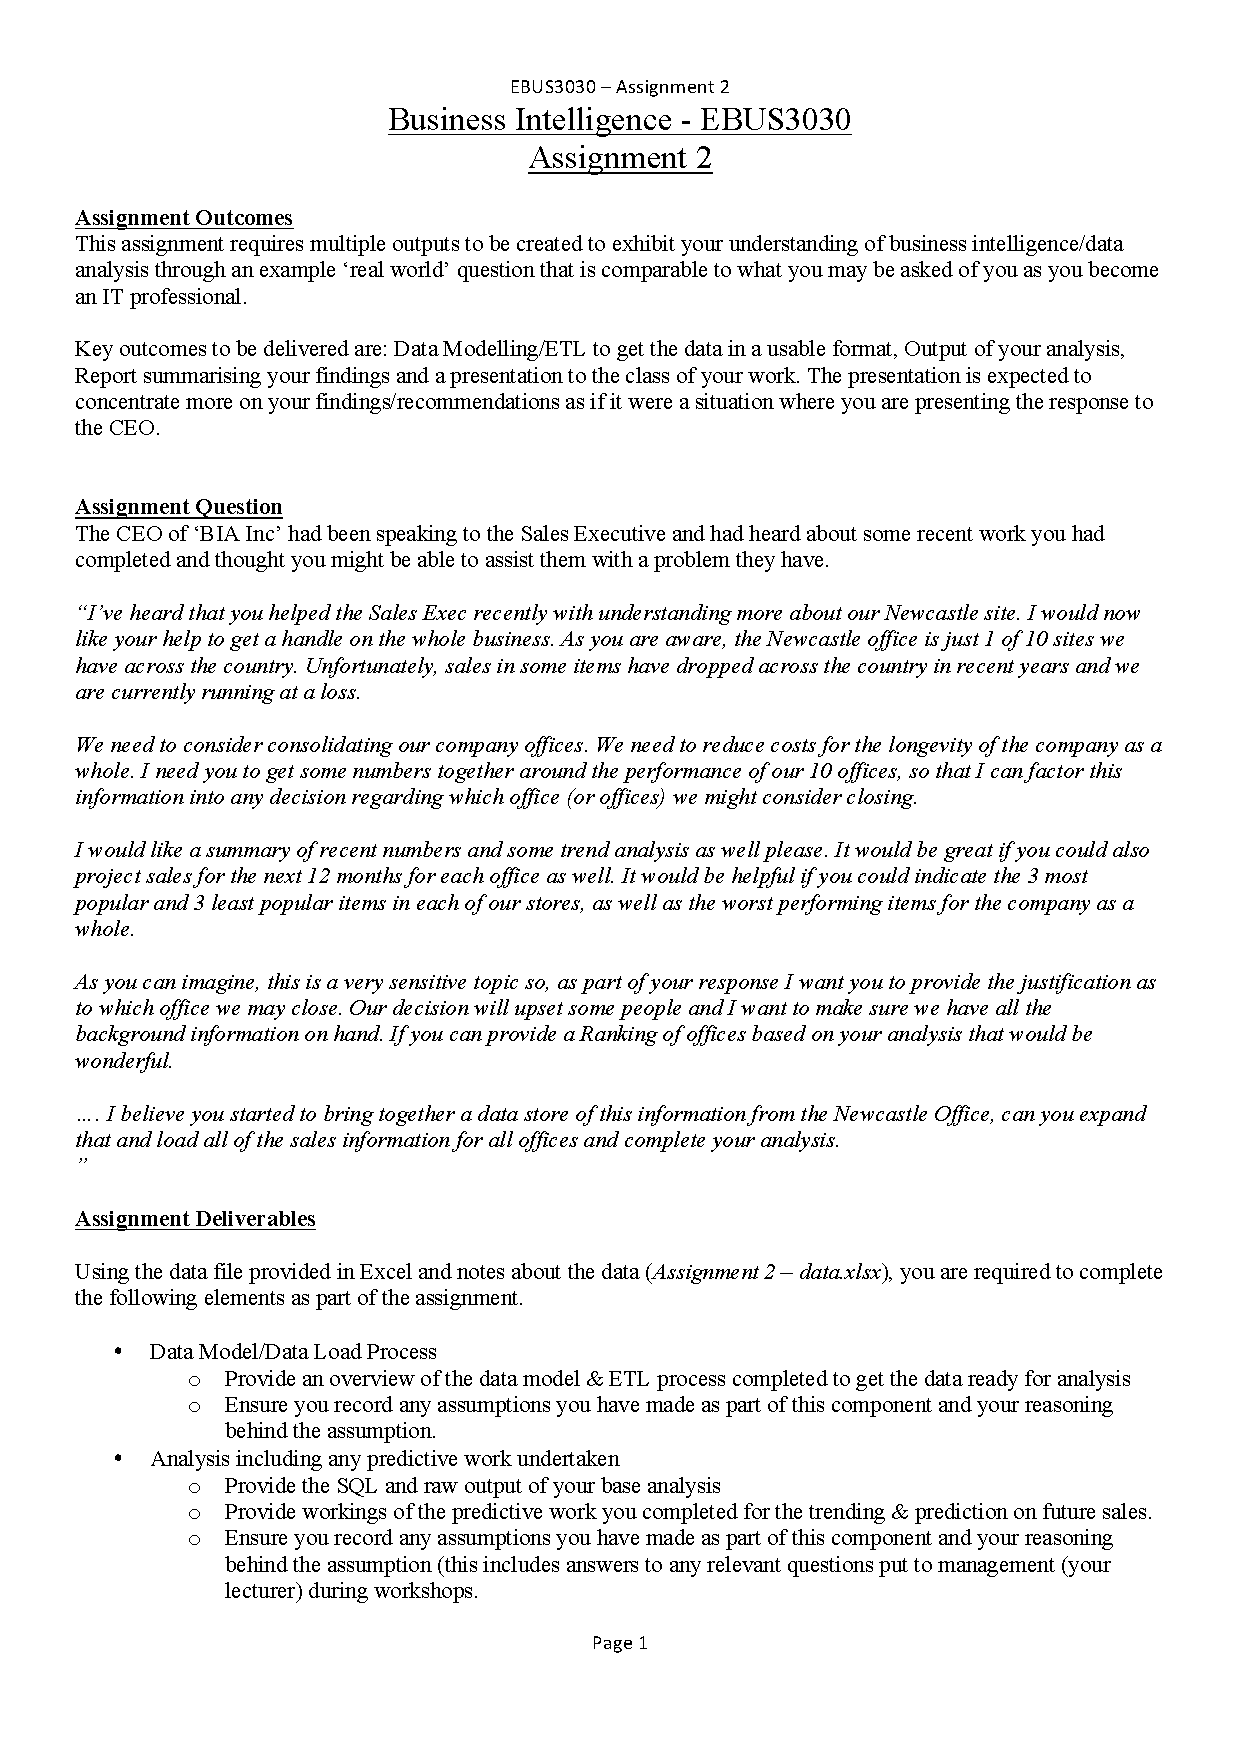
\includepdf[pagecommand=\section{Assignment Overview \& Requirements},width=\textwidth,keepaspectratio,pages={1}]{Resources/Assignment_2_Overview.pdf}
    \includepdf[width=\textwidth,keepaspectratio,pages={2}]{Resources/Assignment_2_Overview.pdf}

% ------------------------------------------------------------------------------------------------ %
% EXECUTIVE SUMMARY
% ------------------------------------------------------------------------------------------------ %

    \section{Executive Summary}
    \label{sec:Executive Summary}
	
    \newpage


% ------------------------------------------------------------------------------------------------ %
% BUSINESS RULES
% ------------------------------------------------------------------------------------------------ %

    \subsection{Datamart Business Rules}
    The following business rules were provided to be used in the context of this assignment:
    \begin{itemize}
        
        \item At BIA all customers interacts are in an online environment, all orders are electronic.
        \item Returning customers can provide POI information via the web interface and look up their
        record and that will flow with the sale.
        \item The sales associate can complete the order form/sale for the client.
        \item Each sale will have a receipt number/id.
        \item A receipt can have many line items.
        \item Each line item can only be for a single item, but the customer can purchase multiples 
        of the same item.
        \item Where a customer has multiple line items, any sale with 5 or more row items 
        (containing at least five (5) different items) is provided a 5\% discount.
        \item The system automatically handles the total for the sale by looking up the item, then 
        multiplying the costs per item by number purchased, and then should store this final field 
        total as a record in the system (but should also be able to see clearly sales that were 
        provided a discount. 
        \item Item prices can change at any point, and the price the customer
        pays is the amount listed for the item on the sale date. We need to
        keep a record of all item prices historically so that we can determine what the store item 
        price was at any particular past date.
        \item Only one (1) BIA sales assistant can be attributed to any receipt.
        \item Customers may visit multiple stores for purchases (ie they are not locked to a particular 
        store). As a result, all customer records are replicated across all stores, so they do not need 
        to be re-recorded at a store by store level.
    \end{itemize}
   
    With these considerations in mind, the following report was created to outline
    the discovery, creation and polish to satisfy the assignment requirements.




% ------------------------------------------------------------------------------------------------ %
% DATA MODEL
% ------------------------------------------------------------------------------------------------ %

    \newpage
    \section{Data Model}
    The below data model is only a suggestion and is still subject to change into the future. A full create script can be found in the \hyperref[sec:Appendix]{\color{blue}appendix}
        \begin{center}
            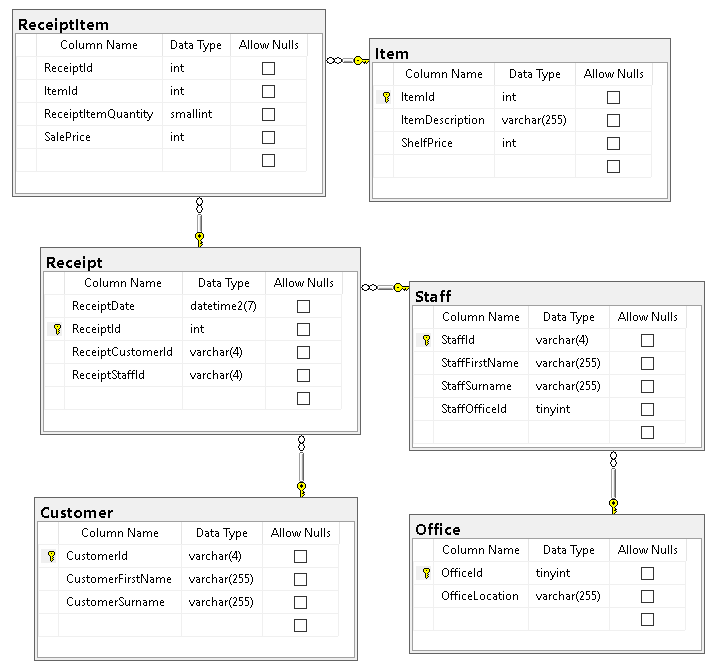
\includegraphics[width=\textwidth,keepaspectratio]{Images/schema.PNG}
        \end{center}
    It must be noted that the structure of this data model is 
    less than efficient, and it would be expected in a datamart
    situation that only at lower levels of data would this schema
    remain responsive in the manner it is now, as the outline
    suggests the datamart is not necessarily the most suitable
    design for future use, however suits very well currently.
    \par
    It would be expected that only at extremely large data sets
    would this model prove a bad design. In such cases a model 
    more representative of the snowflake or star schema would be
    heavily advised.

    \newpage
    An EER diagram of the suggested data model:
    \begin{center}
        %\includegraphics[width=\textwidth-40pt,keepaspectratio]{Images/EER_diagram.png}
    \end{center}



% ------------------------------------------------------------------------------------------------ %
% DATA LOAD PROCESS
% ------------------------------------------------------------------------------------------------ %

    \newpage
    \section{Data Load Process (ETL/ELT)}
        Initial import of the data supplied in the xlsx file generated a very basic table
        that allowed us to analyze the data for potential outliers, confirm the business
        requirements of the data and then create tables from which the data model was derived.
        \\
        The Imported table structure was as follows:
        \begin{center}
            %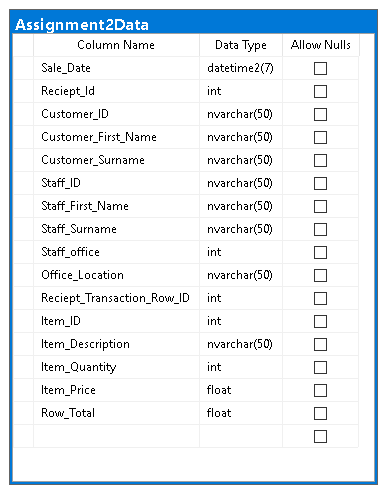
\includegraphics{Images/Initial_Import.PNG}
        \end{center}

        \noindent
        A decision to leave this initial import table as default
        was made to allow easy reference to the initially supplied
        excel data file.
        % \par
        % In the following sections of \hyperref[sec:QAP]{\color{blue}Quality Assurance Processes}, \hyperref[sec:AR]{\color{blue}Assumptions and Reasoning} and \hyperref[sec:BA]{\color{blue}Base Analysis} we intend to clarify the reasoning behind leaving the imported data in
        % the default table suggested by SSMS.

        \newpage



% ------------------------------------------------------------------------------------------------ %
% QA PROCESS
% ------------------------------------------------------------------------------------------------ %

        \subsection{Quality Assurance Processes}
        \label{sec:QAP}
            Maybe include some C\# code references or whatnot.
% ------------------------------------------------------------------------------------------------ %
% ASSUMPTIONS/REASONING
% ------------------------------------------------------------------------------------------------ %

        \newpage
        \subsection{Assumptions and Reasoning}
        \label{sec:AR}
            \subsubsection{Item}

            \subsubsection{ReceiptItem}

            \subsubsection{Receipt}

            \subsubsection{Staff}

            \subsubsection{Customer}

            \subsubsection{Office}

% ------------------------------------------------------------------------------------------------ %
% BASE ANALYSIS
% ------------------------------------------------------------------------------------------------ %
    \section{Base Analysis}
    \label{sec:BA}

        \subsection{Notes on Analysis}

            \subsection{Raw Results}

            % A number of metrics were considered to satisfy the request related to the best salesperson,
            % as we are not certain if this is determined by a specific metric or a set of metrics we 
            % included a number of analyzed points for the project:
            % \begin{itemize}
            %     \item Total receipts attributed to a staff member
            %     \item Total items sold by a staff member
            %     \item Ratio of discounted sales to normal sales for each staff member
            %     \item Total sale value per staff member
            %     \item Average sale value per staff member
            %     \item Average item value per staff member
            % \end{itemize}

                \newpage

            \subsubsection{Total Number of Sales}
                % The total number of sales per staff member were considered with the following 
                % sql query:
                % \begin{lstlisting}
                %     -- Sales count per staff member (Receipt Count)
                %     SELECT COUNT(*) AS 'Sales Count', s.StaffId,s.StaffFirstName,s.StaffSurname
                %     FROM Receipt r
                %     INNER JOIN ReceiptItem ri ON r.ReceiptId = ri.ReceiptId
                %     INNER JOIN Item i ON i.ItemId = ri.ItemId
                %     INNER JOIN Price p ON p.PriceId = ri.PriceId
                %     INNER JOIN Staff s ON s.StaffId = r.ReceiptStaffId
                %     GROUP BY s.StaffId,s.StaffFirstName,s.StaffSurname
                %     ORDER BY 'Sales Count' DESC;
                % \end{lstlisting}

            \subsubsection{Total Items Sold}
                % The total items attributed to each staff member were considered also,
                % determined by the query:
                
                % \begin{lstlisting}
                %     -- Item count per staff member
                %     SELECT SUM(ri.ReceiptItemQuantity) AS 'Item Count', s.StaffId,s.StaffFirstName,s.StaffSurname
                %     FROM Receipt r
                %     INNER JOIN ReceiptItem ri ON r.ReceiptId = ri.ReceiptId
                %     INNER JOIN Staff s ON s.StaffId = r.ReceiptStaffId
                %     GROUP BY s.StaffId,s.StaffFirstName,s.StaffSurname
                %     ORDER BY 'Item Count' DESC;
                % \end{lstlisting}

                % Yielding a range of 4217 to 2813, with the top five staff members in this
                % analysis:

            \newpage
            \subsubsection{Discounted Sales Ratio}
                % Consideration of the number of sales made by each staff member was also made,
                % the following query yielding the results we required:

            % \begin{lstlisting}
            %     -- Sales metrics for discounted and standard sales per staff member
            %     SELECT s.StaffId,s.StaffFirstName,s.StaffSurname,
            %     SUM(SubQuery.[Discounted Sales]) AS 'Discounted Sales',
            %     SUM(SubQuery.[Standard Sales]) AS 'Standard Sales'
            %     FROM (
            %         SELECT CAST(
            %             CASE
            %             WHEN COUNT(ri.[ReceiptItemQuantity]) >= 5
            %                 THEN 1
            %             ELSE 0
            %             END AS int) AS 'Discounted Sales',
            %         CAST(
            %             CASE
            %             WHEN COUNT(ri.[ReceiptItemQuantity]) >= 5
            %                 THEN 0
            %             ELSE 1
            %         END AS int) AS 'Standard Sales',
            %         r.ReceiptId
            %         FROM Receipt r
            %         INNER JOIN ReceiptItem ri ON r.ReceiptId = ri.ReceiptId
            %         INNER JOIN Item i ON i.ItemId = ri.ItemId
            %         INNER JOIN Price p ON p.PriceId = ri.PriceId
            %         GROUP BY r.ReceiptId
            %     ) AS SubQuery
            %     INNER JOIN Receipt r ON SubQuery.ReceiptId = r.ReceiptId
            %     INNER JOIN ReceiptItem ri ON r.ReceiptId = ri.ReceiptId
            %     INNER JOIN Staff s ON s.StaffId = r.ReceiptStaffId
            %     GROUP BY s.StaffId,s.StaffFirstName,s.StaffSurname
            % \end{lstlisting}

            \newpage
            \subsubsection{Total Sales Value per Staff Member}

            % Consideration of the total sales per staff member was considered a highly important 
            % metric to consider also, we did consider comparing the results of this to the 
            % results of a query that did not include discount to see whom would be considered
            % the best performer if discounts were not relevant, however we also recognise this to be too
            % speclutive in nature. The required query was as follows:

            % \begin{lstlisting}
            % -- Sales total per staff with discounts applied ($)
            % SELECT CAST(
            %         CASE
            %         WHEN COUNT(ri.[ReceiptItemQuantity]) >= 5
            %             THEN SUM(p.[Price] * ri.[ReceiptItemQuantity]) * 0.85
            %         ELSE SUM(p.[Price] * ri.[ReceiptItemQuantity])
            %         END AS decimal(19,5)) AS 'Sales Totals',
            %         s.StaffId,s.StaffFirstName,s.StaffSurname
            % FROM Receipt r
            % INNER JOIN ReceiptItem ri ON r.ReceiptId = ri.ReceiptId
            % INNER JOIN Item i ON i.ItemId = ri.ItemId
            % INNER JOIN Price p ON p.PriceId = ri.PriceId
            % INNER JOIN Staff s ON s.StaffId = r.ReceiptStaffId
            % INNER JOIN Customer c ON c.CustomerId = r.ReceiptCustomerId
            % GROUP BY s.StaffId,s.StaffFirstName,s.StaffSurname
            % ORDER BY 'Sales Totals' DESC;
            % \end{lstlisting}

            \newpage

            \subsubsection{Average Value Per Sale}

            % The average receipt value per staff member was another metric we considered would add
            % value to the descision to be suggested in the 
            % \hyperref[sec:Executive Summary]{\color{blue}executive summary}.
            % The required query to determine this metric was as follows:

            % \begin{lstlisting}
            % -- Sales average per staff with discounts applied
            % SELECT (CAST(
            %         CASE
            %         WHEN COUNT(ri.[ReceiptItemQuantity]) >= 5
            %             THEN SUM(p.[Price] * ri.[ReceiptItemQuantity]) * 0.85
            %         ELSE SUM(p.[Price] * ri.[ReceiptItemQuantity])
            %         END AS decimal(19,5)) / COUNT(r.ReceiptId)) AS 'Sales Average',
            %         s.StaffId,s.StaffFirstName,s.StaffSurname
            % FROM Receipt r
            % INNER JOIN ReceiptItem ri ON r.ReceiptId = ri.ReceiptId
            % INNER JOIN Item i ON i.ItemId = ri.ItemId
            % INNER JOIN Price p ON p.PriceId = ri.PriceId
            % INNER JOIN Staff s ON s.StaffId = r.ReceiptStaffId
            % GROUP BY s.StaffId,s.StaffFirstName,s.StaffSurname
            % ORDER BY 'Sales Average' DESC;
            % \end{lstlisting}

            % \par\noindent
            % Outlier: We recognise that Amber Hill (S3) has the highest Average Sale Total, 
            % this is backed up by his very high 
            % Item sales count, showing she is making more sales per Receipt on average 
            % than any other sales Officer. However She has not made as much revenue as 
            % some other employees, about \$7.5k behind the most sales at \$78,572. We 
            % suspected that maybe she was a new employee but after looking at her
            % sale receipt dates we can confirm this is inacurate and that she was 
            % working within the business throughout the entirety of 2017. After learning that she 
            % is not a new employee we can rule the possibility of her being the best 
            % salesperson out. The data suggests that she has been selling higher cost items to make up 
            % the lack of transactions shes involed in compared to others. This is 
            % negligable however since she is under performing compared to others anyway. 

            % With results as follows:

            % We consider this to be a metric which weighs heavily in our analysis,
            % as multiple factors would impact this result, the number of items on the sale
            % (resulting in a lower total if discount was applied). Another consideration 
            % for this metric would be that it leans towards anyone who could
            % sell a larger quantity of the same item, as this lends itself towards a higher
            % receipt total. 
			
			% \par
			% We see that Ms Amber Hill (S3) has the highest average sale total and this is backed up by
			% her high item sales count, indicating she is making more sales per receipt on average than
			% any other sales office. 
			% However, Ms Hill has not made as much revenue as some other employees, approximately \$7,500
			% behind the sales leader who achieved \$78,572. Originally, we suspected that perhaps Ms Hill
			% was a new employee but reviewing sale receipt dates we can confirm this was not a valid
			% assumption and that she was working within the business throughout the entirety of 2017.
			% After this revelation, we can rule Ms Hill out of our assessment for the best sales person.
			% The data suggests that Ms Hill sells higher cost items which makes up for the lack of
			% transactions she completes when compared to other staff members. 


% ------------------------------------------------------------------------------------------------ %
% CONCLUSION & RECOMMENDATIONS
% ------------------------------------------------------------------------------------------------ %
	\newpage
    \section{Conclusion and Recommendations}
            % This report is designed to identify the best performing Sales Officer at BIA Inc by 
            % directive of the Head Sales Executive of BIA Inc.
            % After considering multiple data points from the newly created Sales Database, 
            % using sales data from 2017 supplied to us by the Head Sales Executive of BIA Inc.
            % We conclude that the Best Sales Officer is Mrs Michelle Miller (S8) becasue she 
            % has a sales total of \$78,572.22 more than \$4k more than the second highest 
            % revenue maker Mrs Kaitlyn Ortiz (S19).
            % She does not have the Highest transaction count however because she has sold 
            % more higher value items this makes up for it. She has sold 4144 compared to 
            % the highest count of 4217. It works out to be a 73 item difference.
            % We beleive that the in excess of \$4k extra that Mrs Michelle Miller brings 
            % to the company out weighs the value of selling 73 extra items. 
            % There for we recommend Mrs Michelle Miller for the reward as the best Sales 
            % Officer at BIA Inc. In the event that  Mrs Michelle Miller is not applicable
            % we would reccomend Mrs Kaitlyn Ortiz whom has 
			% achieved a high evaluation from all the data points that we analyzed.

% ------------------------------------------------------------------------------------------------ %
% REFERENCES
% ------------------------------------------------------------------------------------------------ %
    
    \newpage
    \begin{thebibliography}{9}
        \raggedright
        \bibitem{MoneyIssues}
            Reasons against TSQL Money type: Stackoverflow User; \textit{SQLMenace}
            \url{https://stackoverflow.com/questions/582797/should-you-choose-the-money-or-decimalx-y-datatypes-in-sql-server}
        \bibitem{Numeric}
            Microsoft TSQL documentation of Decimal/Numeric types
            \url{https://docs.microsoft.com/en-us/sql/t-sql/data-types/decimal-and-numeric-transact-sql?view=sql-server-2017}
        \bibitem{CTE}
        Microsoft documentation: WITH common\_table\_expression (Transact-SQL)
            \url{https://docs.microsoft.com/en-us/sql/t-sql/queries/with-common-table-expression-transact-sql?view=sql-server-2017}
        \bibitem{BusDictionairyUpselling}
        		Upselling - Business Dictionary
        		\url{http://www.businessdictionary.com/definition/upselling.html}
    \end{thebibliography}

% ------------------------------------------------------------------------------------------------ %
% APPENDIX
% ------------------------------------------------------------------------------------------------ %

    \newpage
    \section{Appendix}
    \label{sec:Appendix}
    
    \end{document}